\documentclass[openany, 11pt]{book}
\makeindex

\usepackage{amsmath}
\usepackage{amssymb}
\usepackage{booktabs}
\usepackage{csvsimple-l3}
\usepackage{bussproofs}
\usepackage{dirtytalk}
\usepackage[dvipsnames]{xcolor}
\usepackage{enumitem}
\usepackage{epigraph}
\usepackage{forest}
\usepackage{formal-grammar}
\usepackage{graphicx}
\usepackage[citecolor=blue,colorlinks=true, linkcolor=blue, urlcolor=blue]{hyperref}
\usepackage{kantlipsum}
\usepackage{makeidx}
\usepackage[margin=0.8in]{geometry}
\usepackage{mathrsfs}
\usepackage[outputdir=../build]{minted}
\usepackage{multicol}
\usepackage[mode=tex]{standalone}
\usepackage[style=authortitle]{biblatex}
\usepackage[T1]{fontenc}
\usepackage[tableaux]{prooftrees}
\usepackage{tcolorbox}
\usepackage{tikz}
\usepackage{titlesec}
\usepackage{xcolor}

\usetikzlibrary{arrows}
\usetikzlibrary{arrows.meta}
\usetikzlibrary{automata}
\usetikzlibrary{calc}
\usetikzlibrary{fit}
\usetikzlibrary{petri}
\usetikzlibrary{positioning}

\tcbuselibrary{breakable}
\tcbuselibrary{listings}
\tcbuselibrary{minted}
\tcbuselibrary{skins}
\tcbuselibrary{theorems}

\newcounter{filePrg}

\addbibresource{biblio.bib}
\setlength{\parindent}{0pt}

\renewcommand{\emph}[1]{\textit{#1}}
\setlength{\parindent}{0pt}

\newcommand\setboxcounter[2]{\setcounter{tcb@cnt@#1}{#2}}
\newcommand\qed[0]{\blacksquare}
\setlength{\parindent}{10pt}
\newcommand{\set}[1]{\{#1\}}
\newcommand{\up}[1]{ \left\lceil#1\right\rceil }
\newcommand{\down}[1]{ \left\lfloor#1\right\rfloor}

\definecolor{CaribbeanBlue}{RGB}{0, 206, 209} % Define Caribbean Blue
\NewTcbTheorem[list inside=definition]{definition}
{Definition}{
	breakable,
	colback=CaribbeanBlue!05,
	colframe=CaribbeanBlue!35!black,
	fonttitle=\bfseries}{th}

\NewTcbTheorem[list inside=intuition]{intuition}{Intuition}{
	breakable,
	colback=blue!5,
	colframe=blue!35!black,
	fonttitle=\bfseries}{th}

\NewTcbTheorem{example}{Example}{
	breakable,
	colback=white,
	colframe=green!35!black,
	fonttitle=\bfseries}{th}

\NewTcbTheorem{verify}{Verify}{
	breakable,
	float,
	colback=red!5,
	colframe=red!35!black,
	fonttitle=\bfseries}{th}

\NewTcbTheorem[list inside=theorem]{theorem}{Theorem}{
	breakable,
	colback=gray!10,
	colframe=gray!35!black,
	fonttitle=\bfseries}{th}

% \NewTcbTheorem[
% list inside=exercise,
% number within=chapter,
% number within=section,
% ]

\NewTcbTheorem[
	list inside=exercise,
	number within=section,
]{exercise}{Exercise}{
	breakable,
	colback=white,
	colframe=black,
	fonttitle=\bfseries}{th}

\newcommand{\hask}[1]{\mintinline{haskell}{#1}}

\newenvironment{alist}
{\begin{enumerate}[label={*}, leftmargin=*, itemsep=0pt, parsep=0pt]}
		{\end{enumerate}}

\newenvironment{blist}
{\begin{enumerate}[label={}, leftmargin=*, itemsep=0pt, parsep=0pt]}
		{\end{enumerate}}

\renewcommand{\thesection}{\arabic{section}}
\tcbset{enhanced jigsaw}

\newtcbinputlisting{\codeFromFile}[2]{
	listing file={#1},
	listing engine=minted,
	minted style=colorful,
	minted language=haskell,
	minted options={breaklines,linenos,numbersep=3mm},
	colback=blue!5!white,colframe=blue!75!black,listing only,
	left=5mm,enhanced,
	title={#2},
	overlay={\begin{tcbclipinterior}\fill[red!20!blue!20!white] (frame.south west)
				rectangle ([xshift=5mm]frame.north west);\end{tcbclipinterior}}
}

\newtcblisting{haskell}[1]
{
	listing engine=minted,
	minted style=colorful,
	minted language=haskell,
	minted options={breaklines,linenos,numbersep=3mm},
	colback=blue!5!white,colframe=blue!75!black,listing only,
	left=5mm,enhanced,
	title={#1},
	overlay={\begin{tcbclipinterior}\fill[red!20!blue!20!white] (frame.south west)
				rectangle ([xshift=5mm]frame.north west);\end{tcbclipinterior}}
}

\title{Boof Proof}
\author{Idris}
\date{March 2024}


\begin{document}
\maketitle{}
\tableofcontents
% \tcblistof[\section]{definition}{List of Definitions}
% \listoffigures
% \listoftables

\part{Fundamentals}
% \chapter{Sets}
% \chapter{Logic}
\setcounter{chapter}{2}
\chapter{Counting}
\setcounter{section}{1}
\section{Multiplication Principle}
\begin{exercise}{}{}
	Consider lists made from the letters T, H, E, O, R, Y,
	with repetition allowed.
	\begin{enumerate}[label = {(\arabic*)}]
		\item How many length-4 lists are there? \\
		      $6^4$
		\item How many length-4 lists are there that begin with T?\\
		      $1 \cdot 6^3$
		\item How many length-4 lists are there that do not begin with T?\\
		      $5 \cdot 6^3$
	\end{enumerate}
\end{exercise}

\begin{exercise}{}{}
	Airports are identified with 3-letter codes. For example,
	Richmond, Virginia has the code RIC, and Memphis, Tennessee has MEM. How
	many different 3-letter codes are possible?
	\begin{enumerate}[label = {(\arabic*)}]
		\item $26^3$
	\end{enumerate}
\end{exercise}

\begin{exercise}{}{}
	How many lists of length 3 can be made from the symbols A,
	B, C, D, E, F if\ldots
	\begin{enumerate}[label = {(\arabic*)}]
		\item repetition is allowed.
		      $ 6^3$
		\item repetition is not allowed.
		      $ 6\cdot 5 \cdot 4$
		\item repetition is not allowed and the list must contain the letter A.
		      $ 6\cdot 5 \cdot 3$
		\item repetition is allowed and the list must contain the letter A.
		\item Let $A=$ list of all length-three strings.
		      Let $B=$ list of all length-three strings without A.
		      Then $|A| - |B| = 6^3 - 5^3$
	\end{enumerate}
\end{exercise}

\begin{exercise}{}{}
	In ordering coffee you have a choice of regular or decaf; small, medium or
	large; here or to go. How many different ways are there to order a coffee?
	\begin{enumerate}[label = {(\arabic*)}]
		\item Let $A = \{\text{regular}, \text{decaf}\}$.
		      Let $B = \{\text{small}, \text{medium}, \text{large}\}$.
		      Let $C = \{\text{here}, \text{to-go}\}$.
		      Different ways to order is the product $|A|\cdot|B|\cdot|C| = 2 \cdot 3 \cdot 2$.
	\end{enumerate}
\end{exercise}

\begin{exercise}{}{}
	This problem involves 8-digit binary strings such as 10011011 or 00001010
	(i.e., 8-digit numbers composed of 0's and 1's).
	\begin{enumerate}[label = {(\alph*)}]
		\item How many such strings are there?
		      There are $2^8$ different 8-digit binary strings.
		\item How many such strings end in 0?
		      There are $2^7$ different 8-digit binary strings that end in $0$.
		\item How many such strings have 1's for their second and fourth digits?
		      There are $2^6$ different 8-digit binary strings that have two of
		      their bits constant.
		\item How many such strings have 1's for their second or fourth digits?
		      Here we must be careful not to double count.
		      Let $A =$ 8-digit strings with 1 as the fourth digit.
		      Let $B =$ 8-digit strings with 1 as the second digit.
		      Let $C =$ 8-digit strings with 1 as the second digit and 1 as the
		      fourth digit.
		      The total number of 8-digit strings with 1 as the second or fourth
		      digit is $|A| + |B| - |C| = 2^7+2^7-2^6$.
	\end{enumerate}
\end{exercise}

\begin{exercise}{}{}
	You toss a coin, then roll a dice, and then draw a card
	from a 52-card deck.
	\begin{enumerate}[label = {(\arabic*)}]
		\item Let $A = \{\text{H}, \text{T}\}$
		      Let $B = \{1, 2, 3, 4, 5, 6\}$
		      Let $C = \{1\ldots 52 \}$
		      How many different outcomes are there?
		      $|A| \cdot |B| \cdot |C| = 2 \cdot 6 \cdot 52$.
		\item How many outcomes are there in which the dice lands on $3$?
		      $|A| \cdot |C| = 2 \cdot 52$.
		      How many outcomes are there in which the dice lands on an odd number?
		      $|A| \cdot |\text{odd}| \cdot |C| = 2 \cdot 3 \cdot 52$.
		\item How many outcomes are there in which the dice lands on an odd number
		      and the card is a King?
		      $|A| \cdot |\text{odd}| \cdot |\text{King}| = 2 \cdot 3 \cdot 4$.
	\end{enumerate}
\end{exercise}

\begin{exercise}{}{}
	This problem concerns 4-letter codes made from the letters A, B, C, D,
	$\ldots$ Z.
	\begin{enumerate}[label = {(\arabic*)}]
		\item How many such codes can be made?
		      $26^4$, assuming repetitions.
		\item How many such codes have no two consecutive letters the same?
		      We can pick any letter to be the first one. To assure a non-consecutive
		      2nd letter, we can pick from 25 letters.  To pick a 3rd letter which is
		      non-consecutive with the 2nd letter, there are 25 choices, as it is now ok
		      to re-use the first letter. And so it goes, so that for every non-first
		      letter, there are $n-1$ choices.
		      Therefore the answer is $26\cdot 25^3$.
	\end{enumerate}
\end{exercise}

\begin{exercise}{}{}
	A coin is tossed 10 times in a row. How many possible
	sequences of heads and tails are there?
	$2^{10}$
\end{exercise}

\begin{exercise}{}{} A new car comes in a choice of five colors, three engine
	sizes and two transmissions. How many different combinations are there?
	$5 \cdot 3 \cdot 2$.
\end{exercise}

\begin{exercise}{}{}
	A dice is tossed four times in a row. There are many
	possible outcomes. How many different outcomes are possible?
	$6^4$
\end{exercise}

\section{Addition and Subtraction Principles}
\begin{exercise}{}{}
	Five cards are dealt off of a standard 52-card deck and
	lined up in a row.
	\begin{itemize}
		\item How many such lineups are there that have at least one red card?
		      Let $A=$ list of all lineups
		      Let $B=$ list of all lineups without a red.
		      Let $C=$ list of all lineups with at least one red.
		      Therefore $|A| - |B| = |C| = \dfrac{52!}{47!} - \dfrac{26!}{21!}$
		\item How many such lineups are there in which the cards are either all
		      black or all hearts?
		      Let $A=$ list of all blacks.
		      Let $B=$ list of all hearts.
		      Let $A \cap B= \emptyset$, because hearts are red.
		      Therefore $|A|+ |B| =\dfrac{26!}{21!} + \dfrac{13!}{8!}$.
	\end{itemize}
\end{exercise}

\begin{exercise}{}{}
	Five cards are dealt off of a standard 52-card deck and lined up in a row.
	How many such lineups are there in which all 5 cards are of the same suit?

	$4 \cdot \dfrac{13!}{8!}$
\end{exercise}

\begin{exercise}{}{}
	Five cards are dealt off of a standard 52-card deck and lined up in a row. How many such lineups are there in which all 5 cards are of the same color (i.e., all black or all red)?
	$2 \cdot \dfrac{26!}{21!}$
\end{exercise}

\begin{exercise}{}{}
	Five cards are dealt off of a standard 52-card deck and lined up in a row.
	How many such lineups are there in which exactly one of the 5 cards is a
	queen?

	$4 \cdot \dfrac{48!}{44!}$
\end{exercise}

\begin{exercise}{}{}
	Consider the integers between 1 and 9999.
	\begin{enumerate}[label = {(\arabic*)}]
		\item How many have no repeated digits?
		      Let $A=1\ldots 9$
		      Let $B=0\ldots 9$
		      For the integers $1\ldots 9$, we can pick any element from $A$, therefore
		      there are $9$ with non-consecutive digits.
		      For the integers $10\ldots 99$, we can pick any element from $A$, and then
		      and non-matching element from $B$, therefore are $9\cdot9=81$ integers in
		      this range with non-consecutive digits.
		      For the integers $C=100\ldots 999$, we can pick any element from $A$, then
		      any non-matching element from $B$, and then lastly another non-matching
		      element from $B$, therefore there are $9\cdot9\cdot9$ integers in this range
		      with non-consecutive digits.
		      For the integers $C=1000\ldots 9999$, follows the same pattern, therefore
		      there are $9\cdot9\cdot9\cdot9$ integers in this range
		      with non-consecutive digits.
		      The answer is $9^1 + 9^2 + 9^3 + 9^4$.

		\item How many have at least one repeated digit?
		      The set of numbers with at least one repeated digit is the inverse of the
		      above calculated set, namely the set of numbers with no repeated digits.
		      Therefore the answer is $9999 - 9^1 - 9^2 - 9^3 - 9^4$.
	\end{enumerate}
\end{exercise}

\begin{exercise}{}{}
	Consider lists made from the symbols A, B, C, D, E, with repetition allowed.
	\begin{enumerate}[label={}, leftmargin=*, itemsep=0pt, parsep=0pt]
		\item Let $A=\{\text{length-5 lists}\},\quad |A| = 5^5$
		\item Let $B=\{\text{length-5 lists}\mid\text{no repeats}\}, \quad |B| = 5!$
		\item Let $C=\{\text{length-5 lists}\mid\text{at least one repeat}\}$
	\end{enumerate}
	\begin{enumerate}[label = {(\alph*)}]
		\item How many such length-5 lists have at least one letter repeated?
		      Herein it's easiest to use the subtraction princple, and calculate $|A|$
		      and $|B|$ to get $|C|$.
		      $C=A - B, \quad |C| = 5^5 - 5! $
		\item How many such length-6 lists have at least one letter repeated?
		      The same principle applies, therefore the answer is $6^6 - 6!$.
	\end{enumerate}
\end{exercise}

\begin{exercise}{}{}
	A password on a certain site must be five characters long,
	made from letters of the alphabet, and have at least one upper case letter.
	\begin{enumerate}[label={}, leftmargin=*, itemsep=0pt, parsep=0pt]
		\item Let $A=\{\text{length-5 string}\},\quad |A| = 52^5$
		\item Let $B=\{\text{length-5 lists}\mid\text{no upper-case}\}, \quad |B| = 26^5$
		\item Let $C=\{\text{length-5 lists}\mid\text{at least one upper-case}\}$
	\end{enumerate}
	\begin{enumerate}[label = {(\arabic*)}]
		\item How many different passwords are there?
		      $|C| = |A| - |B| = 52^5 - 26^5.$
		\item What if there must be a mix of upper and lower case?
		      \begin{enumerate}[label={}, leftmargin=*, itemsep=0pt, parsep=0pt]
			      \item Let $D=\{\text{length-5 lists}\mid\text{no lower-case}\}, \quad |D| = 26^5$
			      \item Let $E=\{\text{length-5 lists}\mid\text{at least one lower-case, at least one lower-case}\}$
			      \item $|E| = |A| - |B| - |D| = 52^5 - 2\cdot26^5.$
		      \end{enumerate}
	\end{enumerate}
\end{exercise}

\begin{exercise}{}{}
	This problem concerns lists made from the letters A, B, C, D, E, F, G, H, I, J.
	\begin{enumerate}[label = {(\arabic*)}]
		\item How many length-5 lists can be made from these letters if
		      repetition is not allowed and the list must begin with a vowel? $3
			      \cdot 9 \cdot 8 \cdot 7 \cdot 6$.
		\item How many length-5 lists can be made from these letters if
		      repetition is not allowed and the list must begin and end with a
		      vowel? $3 \cdot 8 \cdot 7 \cdot 6 \cdot 2$.
		\item How many length-5 lists can be made from these letters if
		      repetition is not allowed and the list must contain exactly one A?
		      $5 \cdot 8 \cdot 7 \cdot 6 \cdot 5$.
	\end{enumerate}
\end{exercise}

\begin{exercise}{}{}
	Consider lists of length 6 made from the letters A, B, C,
	D, E, F, G, H. How many such lists are possible if repetition is not allowed
	and the list contains two consecutive vowels?
	\begin{enumerate}[label={}, leftmargin=*, itemsep=0pt, parsep=0pt]
		\item Let $X=\{\text{A, B, C, D, E, F, G, H}\}$
		\item Let $Y=\{\text{B, C, D, F, G, H}\}$
		\item All lists that fit the description will contain 2 vowels. First we can
		      calculate the number of ways to arrange the non-vowels from $Y$, which is
		      $6\cdot5\cdot4\cdot3$.
		\item There are then $5$ locations to insert the consecutive vowels, and 2 ways
		      to arrange the consecutive vowels, either AE or EA.
		\item Therefore there are $6\cdot5\cdot4\cdot3 \cdot 5 \cdot 2$ ways to make the
		      specified list.
	\end{enumerate}
\end{exercise}

\begin{exercise}{}{}
	Consider the lists of length six made with the symbols P, R, O, F, S,
	where repetition is allowed. (For example, the following is such a list:
	(P,R,O,O,F,S).) How many such lists can be made if the list must end in an S
	and the symbol O is used more than once?
	\begin{enumerate}[label={\textbullet}, leftmargin=*, itemsep=0pt, parsep=0pt]
		\item Since the last letter must be an S, there are only 5 spots where there are
		      different letters possible.
		\item Therefore the question is transformed into the following: How many
		      \mbox{length-five} lists can be made, with at least two Os.
		\item Let $A=\{\text{length-5 lists}\}$
		\item Let $B=\{\text{length-5 lists}\mid\text{0 O}\}$
		\item Let $C=\{\text{length-5 lists}\mid\text{1 O}\}$
		\item Let $D=\{\text{length-5 lists}\mid\text{at least 2 Os}\}$
		\item $|D| = |A| - |B| - |C|$
		\item $|A| = 5^5$, choose any of the 5 letters, 5 times
		\item $|B| = 4^5$, choose any of the 5 letters other than O, 5 times
		\item $|C| = 4^4 \cdot 5$, choose any length-4 list, and then insert an O in any
		      of the 5 spots
		\item Therefore, $|D| = |A| - |B| - |C| = 5^5 - 4^5 - 4^4 \cdot 5$
	\end{enumerate}
\end{exercise}

\begin{exercise}{}{}
	\begin{enumerate}[label = {(\arabic*)}]
		\item How many integers between 1 and 1000 are divisible by 5?
		      \begin{enumerate}[label={}, leftmargin=*, itemsep=0pt, parsep=0pt]
			      \item There are 1000 numbers in that set, and that set is equally partitioned
			            into 10 subsets by looking at the last digit.
			      \item A number is divisble by 5 if it ends in 0 or 5, which is $\dfrac{1}{5}$ of
			            the set.
			      \item Therefore 200 numbers in the set of integers from 1 to 1000 are divisible
			            \mbox{by 5}.
		      \end{enumerate}
		\item How many are not divisible by 5?
		      The rest, 800.
	\end{enumerate}
\end{exercise}

\begin{exercise}{}{}
	Six math books, four physics books and three chemistry books are
	arranged on a shelf. How many arrangements are possible if all books of the
	same subject are grouped together?
	\begin{enumerate}[label={\textbullet}, leftmargin=*, itemsep=0pt, parsep=0pt]
		\item Within this problem there exists the subproblem of how many ways books of
		      the same subject can be arranged, which is dependent of the size of the set
		      $n$.
		\item Therefore there are $n!$ ways to arrange books of the same category.
		\item Next, we must determine how many ways there are to arrange sets of similar
		      books, and again it is $m!$, where $m$ is the number of subjects.
		\item Therefore there are $m! \cdot n_1! \cdot n_2! \cdot n_3!$ ways to arrange the
		      books, with the constraint that books are grouped together by subject.
		\item Therefore there are $3! \cdot 6! \cdot 4! \cdot 3!$ ways to arrange the
		      books.
	\end{enumerate}
\end{exercise}

\section{Factorials and Permutations}
\begin{exercise}{}{}
	What is the smallest n for which n! has more than 10 digits?
	If a number is 10 digits, then it must be more than $10^{9}$. 13
\end{exercise}

\begin{exercise}{}{}
	For which values of $n$ does $n!$ have n or fewer digits?
	\begin{enumerate}[label={\textbullet}, leftmargin=*, itemsep=0pt, parsep=0pt]
		\item Let $f$ be a function return the number of digits of a number
		\item From the above question we know that $10 < f(13!) < 11$.
		\item Now $14!$, will add least one more digit, and at some point around
		      15 or 16 I think.
		\item Just use a calculator, or stirling's approximation.
	\end{enumerate}
\end{exercise}

\begin{exercise}{}{}
	How many 5-digit positive integers are there in which there are no repeated
	digits and all digits are odd?
	\begin{enumerate}[label={\textbullet}, leftmargin=*, itemsep=0pt, parsep=0pt]
		\item There are 5 digits to work with, namely the odd digits.
		\item There are $5!$ such numbers, which are positive integers, in which
		      no digit is repeated, the number is odd, and each digit is odd.
	\end{enumerate}
\end{exercise}

\begin{exercise}{}{}
	Using only pencil and paper, find the value of $\dfrac{100!}{95!}$.

	Yeah, no.
\end{exercise}

\begin{exercise}{}{}
	Using only pencil and paper, find the value of $\dfrac{120!}{118}$.

	Yeah, no.
\end{exercise}

\begin{exercise}{}{}
	There are two 0's at the end of $10! = 3,628,800$. Using
	only pencil and paper, determine how many 0's are at the end of the number
	100!.
	\begin{enumerate}[label={\textbullet}, leftmargin=*, itemsep=0pt, parsep=0pt]
		\item Each time the quantity $10!$ is multiplied by $10$, another $0$ will be
		      appended to the end of the number.
		\item We can factor out primes from the elements of the set 11-100, with the goal
		      of factoring out 2s and 5s, so they can multiply together to get
		      $2\cdot5=10$.
		\item Between 11 and 100, 17 numbers are divisible by 5 (15, 20, ...100), and 3
		      of them have 5 as a factor twice (25, 75, 100). Therefore we have 20 5's.
		\item It's obvious there are at least 20 2's available in the range, so in total
		      we can pair 5 and 2 together 20 times.
		\item Each time we multiply by 2 and 5, we add another zero.
		\item Therefore there will 20 be additional zeroes, for a total of 22 zeroes at the end
		      of 100!.
	\end{enumerate}
\end{exercise}

\begin{exercise}{}{}
	Find how many 9-digit numbers can be made from the digits 1, 2, 3, 4, 5, 6, 7,
	8, 9 if repetition is not allowed and all the odd digits occur first (on the left)
	followed by all the even digits (i.e., as in 137598264, but not 123456789).

	$5! \cdot 4!$ \square
\end{exercise}

\begin{exercise}{}{}
	Compute how many 7-digit numbers can be made from the digits 1, 2, 3, 4, 5, 6, 7
	if there is no repetition and the odd digits must appear in an unbroken sequence.
	(Examples: 3571264 or 2413576 or 2467531, etc., but not 7234615.)
	\begin{enumerate}[label={\textbullet}, leftmargin=*, itemsep=0pt, parsep=0pt]
		\item First let's calculate the number of ways to create the odd sequence, which
		      is $4!$.
		\item There are 3 evens, therefore there are 4 spots the odd sequence can be
		      interspersed within the evens.
		\item Therefore there are $4\cdot 4!$ to make such a number.
		      \square
	\end{enumerate}
\end{exercise}

\begin{exercise}{}{}
	How many permutations of the letters A, B, C, D, E, F, G
	are there in which the three letters ABC appear consecutively, in
	alphabetical order?
	\begin{enumerate}[label={\textbullet}, leftmargin=*, itemsep=0pt, parsep=0pt]
		\item There are 4 elements not part of the ABC sequence, therefore there are 5
		      spots to insert the ABC sequence.
		\item There the non ABC elements can be arranged in $4!$ permutations.
		\item Therefore there are $4\cdot4!$ ways to make such a sequence.
	\end{enumerate}
\end{exercise}

\begin{exercise}{}{}
	How many permutations of the digits 0, 1, 2, 3, 4, 5, 6, 7, 8, 9 are there
	in which the digits alternate even and odd? (For example, 2183470965.)
	\begin{enumerate}[label={\textbullet}, leftmargin=*, itemsep=0pt, parsep=0pt]
		\item The permutation can start 2 ways, either with an odd or an even.
		\item There 5 possibilties for the 1st spot and 2nd spot, 4 for the 3rd and 4th
		      spot, and so on.
		\item Therefore there are $2\cdot 5!\cdot5!$. possibilities. \square
	\end{enumerate}
\end{exercise}

\begin{exercise}{}{}
	You deal 7 cards off of a 52-card deck and line them up in
	a row. How many possible lineups are there in which not all cards are red?
	\begin{enumerate}[label={\textbullet}, leftmargin=*, itemsep=0pt, parsep=0pt]
		\item Let $A=$ set of all 7 card lineups
		\item Let $B=$ set of all red-only 7 card lineups
		\item Let $C=$ set of all lineups in which not all the cards are red
		\item $|A| - |B| = |C|$
		\item $|A|=\dfrac{52!}{45!}$
		\item $|B|=\dfrac{13!}{6!}$
		\item $|C|=\dfrac{52!}{45!} - \dfrac{13!}{6!}$ \square
	\end{enumerate}
\end{exercise}

\begin{exercise}{}{}
	You deal 7 cards off of a 52-card deck and line them up in
	a row. How many possible lineups are there in which no card is a club?
	\begin{enumerate}[label={\textbullet}, leftmargin=*, itemsep=0pt, parsep=0pt]
		\item For there to be no clubs, we can imagine starting with a deck of 39
		      cards without any clubs.
		\item Therefore the answer is $\dfrac{39!}{32!}$. \square
	\end{enumerate}
\end{exercise}

\begin{exercise}{}{}
	How many lists of length six (with no repetition) can be
	made from the 26 letters of the English alphabet?

	$\dfrac{26!}{20!}$\square
\end{exercise}

\begin{exercise}{}{}
	Five of ten books are arranged on a shelf. In how many ways can this be done?

	Assuming that different orderings of books are considered different
	arrangements, there are $\dfrac{10!}{5!}$ possible arrangements. \square
\end{exercise}

\begin{exercise}{}{}
	In a club of 15 people, we need to choose a president,
	vice-president, secretary, and treasurer. In how many ways can this be done?
	\begin{enumerate}[label={\textbullet}, leftmargin=*, itemsep=0pt, parsep=0pt]
		\item There are 4 different positions, and the order matters, as the positions
		      are not equivalent.
		\item Therefore there are $\dfrac{15!}{11!}$ distinct possible
		      arrangements. \square
	\end{enumerate}
\end{exercise}

\begin{exercise}{}{}
	How many 4-permutations are there of the set A,B,C,D,E,F
	if whenever A appears in the permutation, it is followed by E?
	\begin{enumerate}[label={\textbullet}, leftmargin=*, itemsep=0pt, parsep=0pt]
		\item Let $X=$ 4-permutations with A.
		\item Let $Y=$ 4-permutations without A.
		\item Let $Z=$ all 4-permutations matching the specification.
		\item For the set X, AE will always appear together. Because there are 2
		      remaining elements, there are 3 spots where AE can in interspersed.
		\item Therefore $|X| = 2 \cdot 4\cdot3 = 4!.$
		\item For the set Y, A will not appear by exercise, therefore $|Y| =
			      \dfrac{5!}{1!} = 5!$.
		\item Therefore $|Z| = |X| + |Y| = 4! + 5!$. \square
	\end{enumerate}
\end{exercise}

\begin{exercise}{}{}
	Three people in a group of ten line up at a ticket counter to buy tickets.
	How many lineups are possible?

	$\dfrac{10!}{7!}$
\end{exercise}

\begin{exercise}{}{}
	The gamma function provides a way of extending factorials to numbers
	other than integers. Extra credit: Compute $\pi$ !.

	\begin{align*}
		\Gamma                    & :[0, \infty) \rightarrow \mathbb{R} \\
		\Gamma(x)                 & =\int_0^{\infty} t^{x-1} e^{-t} d t \\
		x \in \mathbb{N}          & \implies \Gamma(x)=(x-1)!           \\
		\forall n \in \mathbb{N}, & \quad n !=\Gamma(n+1)
	\end{align*}

	Check that this is true for $x=1,2,3,4$.
\end{exercise}

\section{Counting Subsets}
\begin{exercise}{}{}
	What is the smallest n for which n! has more than 10 digits?
	\begin{enumerate}[label={\textbullet}, leftmargin=*, itemsep=0pt, parsep=0pt]
		\item If a number is 10 digits, then it must be more than $10^{9}$.
		\item 13
	\end{enumerate}
\end{exercise}

\begin{exercise}{}{}
	Suppose a set A has 37 elements
	\begin{enumerate}[label = {(\arabic*)}]
		\item How many subsets of A have 10 elements?
		      $\dbinom{37}{10} = \dfrac{37!}{27! \cdot10!}$
		\item How many subsets have 30 elements?
		      $\dbinom{37}{30} = \dfrac{37!}{30! \cdot7!}$
		\item How many have 0 elements?
		      $\dbinom{37}{0} = \dfrac{37!}{0! \cdot37!}=1$
	\end{enumerate}
\end{exercise}

\begin{exercise}{}{}
	Suppose A is a set for which $|A| = 100$.
	\begin{enumerate}[label = {(\arabic*)}]
		\item How many subsets of A have 5 elements?
		      $\dbinom{100}{5} = \dfrac{100!}{5! \cdot95!}$
		\item How many subsets have 10 elements?
		      $\dbinom{100}{10} = \dfrac{100!}{10! \cdot90!}$
		\item How many have 99 elements?
		      $\dbinom{100}{99} = \dfrac{100!}{99! \cdot1!}= 100$
	\end{enumerate}
\end{exercise}

\begin{exercise}{}{}
	A set X has exactly 56 subsets with 3 elements. What is the cardinality of X?
	\begin{align*}
		\dbinom{a}{3}            & = \dfrac{a!}{3! \cdot(a-3)!}=56, a \in \mathbb{N}. \\
		\dfrac{(a)(a-1)(a-2)}{6} & =56                                                \\
		(a)(a-1)(a-2)            & =336                                               \\
		a(a^2-3a+2)              & =336                                               \\
		a^3-3a^2+2a              & =336                                               \\
		a^3-3a^2+2a-336          & =0
	\end{align*}
	via the rational root theorem, $a=8$.
\end{exercise}

\begin{exercise}{}{}
	Suppose a set B has the property that
	\begin{enumerate}[label={\textbullet}, leftmargin=*, itemsep=0pt, parsep=0pt]
		\item $$|\{X: X \in \mathcal{P}(B),\quad|X|=6\}|=28$$
		\item Find $|B|$.
		\item B is set such that there 28 subset elements of its powerset that have
		      6 elements.
		\item $\dbinom{a}{6}=28 = \dfrac{a!}{6!\cdot(a-6)!}$
		\item $\dfrac{a(a-1)(a-2)(a-3)(a-4)(a-5)}{6!}=28$
		\item $a(a-1)(a-2)(a-3)(a-4)(a-5)=28\cdot6!$
		\item through trial and error, $a=8$.
	\end{enumerate}
\end{exercise}

\begin{exercise}{}{}
	How many 16-digit binary strings contain exactly seven 1's?
	\begin{alist}
		\item Examples
		\item 0111000011110000
		\item 0011001100110010
		\item $\dbinom{16}{7}= \dfrac{16!}{7!\cdot9!}$
	\end{alist}
\end{exercise}

\begin{exercise}{}{}
	6. $|\{X \in \mathcal{P}(\{0,1,2,3,4,5,6,7,8,9\}):|X|=4\}|=?$
	\begin{alist}
		\item $X$ is a set-element of the powerset of the set comprising the digits 0..9.
		\item $\dbinom{10}{4}= \dfrac{10!}{6!\cdot4!}=210$
	\end{alist}
\end{exercise}

\begin{exercise}{}{}
	$|\{X \in \mathcal{P}(\{0,1,2,3,4,5,6,7,8,9\}):|X|<4\}|=?$
	\begin{alist}
		\item $X$ is a set-element of the powerset of the set comprising the digits 0..9.
		\item $\dbinom{10}{3} + \dbinom{10}{2} + \dbinom{10}{1} + \dbinom{10}{0}$
	\end{alist}
\end{exercise}

\begin{exercise}{}{}
	This problem concerns lists made from the symbols A, B, C, D, E, F, G, H, I.

	\begin{enumerate}[label = {(\arabic*)}]
		\item (a) How many length-5 lists can be made if there is no repetition
		      and the list is in alphabetical order? (Example: BDEFI or ABCGH, but
		      not BACGH.)
		      \begin{alist}
			      \item There is an equivalent problem where we choose 5 letters without
			      replacement. Each such list has a distinct ordering, which is equivalent to
			      a sorted list without replacement.
			      \item Therefore the answer is $\binom{8}{5}=56.$
		      \end{alist}
		\item How many length-5 lists can be made if repetition is not allowed and
		      the list is not in alphabetical order?
		      \begin{alist}
			      \item Here we do not consider each set of the same letters as unique, so we can
			      just the multiplication principle and the answer is $\dfrac{8!}{3!}$.
		      \end{alist}
	\end{enumerate}
\end{exercise}

\begin{exercise}{}{}
	This problem concerns lists of length 6 made from the
	letters A,B,C,D,E,F, without repetition. How many such lists have the
	property that the D occurs before the A?
	\begin{alist}
		\item It is equally likely that D appears before the A as it is the D appears
		after the A.
		\item The number of possible lists is $6!$, and the number of possible list
		where the D appears before the A is $\dfrac{6!}{2}$.
	\end{alist}
\end{exercise}

\begin{exercise}{}{}
	A department consists of 5 men and 7 women. From this
	department you select a committee with 3 men and 2 women. In how many ways
	can you do this?
	\begin{alist}
		\item There $\dbinom{5}{3}$ to choose the men, and $\dbinom{7}{2}$ to choose the
		women.
		\item Therefore there are $\dbinom{5}{3}\cdot \dbinom{7}{2}$ ways to create the
		committee.
	\end{alist}
\end{exercise}

\begin{exercise}{}{}
	How many positive 10-digit integers contain no 0's and exactly three 6's?
	\begin{alist}
		\item First let us determine the slots where the 6s can go. There are 10 slots,
		thus the 6s can go in $\binom{10}{3}$ spots.
		\item Next let us determine the number of digits comprised of 1..5,7..9 that
		are length-7. Since the set has 8 digits, the answer is $8^7$.
		\item Thus by the multiplication principle, where there
		$8^{7}\cdot\binom{10}{3}$ possibilities.
	\end{alist}
\end{exercise}

\begin{exercise}{}{}
	Twenty-one people are to be divided into two teams, the
	Red Team and the Blue Team. There will be 10 people on Red Team and 11
	people on Blue Team. In how many ways can this be done?
	\begin{alist}
		\item Determining one team fully determines the other team. We can use this idea
		to see if we get the same answer, depending on which team is formed first.
		\item To form the blue team, there are $\dbinom{21}{11}$ possibilities.
		\item To form the red team, there are $\dbinom{21}{10}$ possibilities.
		\item $\dbinom{21}{10} = \dfrac{21!}{10!\cdot11!} = \dbinom{21}{11}$, thus we
		can see that forming either team first results in the same answer.
	\end{alist}
\end{exercise}

\begin{exercise}{}{}
	% Suppose $n, k \in \mathbb{Z$, and $0 \leq k \leq n$. Use
	% Fact 3.5, the formula $\left(\begin{array}{c}n \\
	% k\end{array}\right)=\dfrac{n !}{k !(n-k) !}$, to show that
	% $\left(\begin{array}{l}n \\ k\end{array}\right)=\left(\begin{array}{c}n \\
	% n-k\end{array}\right)$.}
	\begin{alist}
		\item $\dbinom{n}{k}=\dfrac{n!}{k!(n-k)!}$
		\item $\dbinom{n}{n-k}=\dfrac{n!}{(n-k)(n-(n-k))!}=\dfrac{n!}{(n-k)!(n-n+k)!}=\dfrac{n!}{(n-k)!k!}$
	\end{alist}
\end{exercise}

\begin{exercise}{}{}
	Suppose $n, k \in \mathbb{Z}$, and $0 \leq k \leq n$. Use Definition 3.2
	alone (without using Fact 3.5) to show that $\left(\begin{array}{l}n \\
				k\end{array}\right)=\left(\begin{array}{c}n \\ n-k\end{array}\right)$.
	\begin{alist}
		\item Suppose some set of cardinality $n$.  Suppose any $k$ such that $0 \leq k \leq n$.
		\item Now we partition $n$ into $k$ and $n-k$ elements. There are two
		equivalent ways of creating this partition, either by selecting $k$ or
		selecting $n-k$ elements.
		\item Therefore $\dbinom{n}{k}$ is equivalent to $\dbinom{n}{n-k}$.
	\end{alist}
\end{exercise}

\begin{figure}
	\centering
	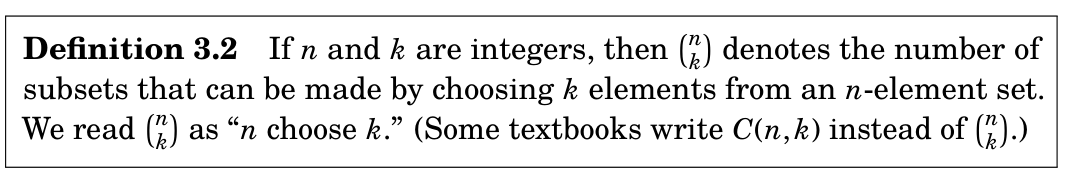
\includegraphics[width=0.9\textwidth]{images/definition03_02.png}
	\label{fig:mypicture}
\end{figure}

\begin{exercise}{}{}
	How many 10-digit binary strings are there that do not have exactly four
	1's?
	\begin{alist}
		\item Let $A=$ set of all 10-digit binary strings.
		\item Let $B=$ set of all 10-digit binary strings with exactly four 1's.
		\item Let $C=$ set of all 10-digit binary strings that do not have exactly
		four 1's.
		\item Because B and C are complements and A is the universe of all 10-digit
		binary strings, then $B \cup C = A$ and $|A|-|B| = |C|$.
		\item Using the multiplication principle, we determine $|A|$ is $2^{10}$.
		\item For $B$, there are 4 spots out of 10 where we can place 1s. Therefore
		\mbox{$|B|=\binom{10}{4}$}.
		\item Therefore $|C|=2^{10} - \binom{10}{4}$.
	\end{alist}
\end{exercise}

\begin{exercise}{}{}
	A = $\{ 0,1,2,3,4,5,6,7,8,9\}$
	\begin{alist}
		\item Let $B=$ Even elements of A.
		\item Let $C=$ Odd elemements of A.
		\item Let $D=$ 6-elements subsets of A that have exactly 3 even elements.
		\item Let $E=$ 6-elements subsets of A that do not have exactly 3 even elements.
		\item How many 6-element subsets of A have exactly three even elements?
		\item We can first choose 3 elements from B, and then choose 3 elements
		of C, and combine them together with the multiplication principle.
		\item $|B| = |C| = \dbinom{5}{3}$, and therefore $|D| = {\dbinom{5}{3}}^2$.
		\item How many do not have exactly three even elements?
		\item E is the complement of D, therefore $|E| = \dbinom{10}{6} -
			{\dbinom{5}{3}}^2$.
	\end{alist}
\end{exercise}

\begin{exercise}{}{}
	Let $A$ be the set of 10-digit binary strings.
	\begin{alist}
		\item Let $B=$ subset of A with exactly four 1's
		\item Let $C=$ subset of A with exactly five 1's
		\item Let $D=$ subset of A whose elements have exactly four 1's or exactly five 1's
		\item Let $E=$ subset of A whose elements do not have exactly four 1's
		or exactly five 1's
		\item How many elements of A are there that have exactly four 1's or exactly five 1's?
		\item Because $B \cap C=\emptyset$, B and C partition D. Therefore, we can
		calculate the cardinalities separately and then add them.
		\item $|B|=\binom{10}{4}$ and $|C|=\binom{10}{5}$, $|D|= \binom{10}{4}+\binom{10}{5}$.
		\item How many do not have exactly four 1's or exactly five 1's?
		\item $E$ is the complemenet of D, therefore $|E| = |A| - |D| = 2^{10} -
			\binom{10}{4}-\binom{10}{5}$.
	\end{alist}
\end{exercise}

\begin{exercise}{}{}
	How many 10-digit binary strings have an even number of 1's?
	\begin{alist}
		\item Let $A$ be the set of 10-digit binary strings.
		\item Let $B=$ subset of A with exactly 0 1's
		\item Let $C=$ subset of A with exactly 2 1's
		\item Let $D=$ subset of A with exactly 4 1's
		\item Let $E=$ subset of A with exactly 6 1's
		\item Let $F=$ subset of A with exactly 8 1's
		\item Let $G=$ subset of A with exactly 10 1's
		\item Let $H=$ subset of A with an even number of 1's
		\item Because B, C, D, E, F, and G partition H, $H=B\cup C\cup D\cup E \cup
			F \cup G$, and therefore $|H|=|B| + |C| + |D| + |E| + |F| + |G|$.
		\item Because of the equivalance of $\binom{n}{k}$ and $\binom{n}{n-k}$,
		$|B|=|G|, |C|=|F|, |D|=|E|$.
		\item Therefore $|H| =
			2\cdot \binom{10}{0} +
			2\cdot \binom{8}{2} +
			2\cdot \binom{6}{4}$.
	\end{alist}
\end{exercise}

\begin{exercise}{}{}
	A 5-card poker hand is called a flush if all cards are the same suit. How
	many different flushes are there?
	\begin{alist}
		\item To get a flush of one particular suit, we choose 5 cards from a set of 13,
		which equals $\dbinom{13}{8}$.
		\item Because there are 4 different suits in the deck of card, we have 4 ways of
		getting the flush and the total number of flush possibilities is $4 \cdot
			\dbinom{13}{8}$.
	\end{alist}
\end{exercise}

\section{Binomial Theorem}
\begin{exercise}{}{}
	Write out row 11 of pascal's triangle.
	\begin{alist}
		\item the first 6 terms of row 11 are unique, and the next fiver terms are mirrors of
		the first five.
		\item the terms of row 11 can be calculated with $\dbinom{11}{i}$, where $i
			\in \mathbb{n}, 0 \leq i \leq 11$.
		\item the $1^{st}$ and $11^{th}$ term of row 11 is
		$\dbinom{11}{0}=\dfrac{11!}{11!\cdot0!}=1$.
		\item the $2^{st}$ and $10^{th}$ term of row 11 is
		$\dbinom{11}{1}=\dfrac{11!}{10!\cdot1!}=11$.
		\item the $3^{rd}$ and $9^{th}$ term of row 11 is
		$\dbinom{11}{2}=\dfrac{11!}{9!\cdot2!}=55$.
		\item the $4^{th}$ and $8^{th}$ term of row 11 is
		$\dbinom{11}{3}=\dfrac{11!}{8!\cdot3!}=165$.
		\item the $5^{th}$ and $7^{th}$ term of row 11 is
		$\dbinom{11}{4}=\dfrac{11!}{7!\cdot4!}=330$.
		\item the $6^{th}$ term of row 11 is
		$\dbinom{11}{5}=\dfrac{11!}{5!\cdot6!}=462$.
	\end{alist}
\end{exercise}

\begin{exercise}{}{}
	Use the binomial theorem to find the coefficient of $x^8 y^5$
	in $(x+ y)^{13}$.
	\begin{alist}
		\item $\dbinom{13}{8}=\dfrac{13!}{8!\cdot5!}\approx 10,00$
	\end{alist}
\end{exercise}

\begin{exercise}{}{}
	Use the binomial theorem to find the coefficient of $x^8$
	in $(x+2)^{13}$.
	\begin{alist}
		\item Let $a=2$, and then $x+2=x+a$
		\item The coefficient of $x^8a^5$ is $\binom{13}{8}$, therefore the coefficient
		of $x^8$ is $2^5\cdot\binom{13}{8}=32\cdot\binom{13}{8}$.
	\end{alist}
\end{exercise}

\begin{exercise}{}{}
	Use the binomial theorem to find the coefficient of $x^6y^3$
	in $(3x-2y)^9$.
	\begin{alist}
		\item Let $a=3x, b=-2y$, and the coefficient for $a^6b^3$ from $(a+b)^9$
		is $\binom{9}{6}$.
		\item Therefore the coeffecient for $x^6y^3$ in $(3x-2y)^9$ is
		$3^6\cdot(-2)^3\cdot\binom{9}{6}$.
	\end{alist}
\end{exercise}

\begin{exercise}{}{}
	Use the binomial theorem to show $\sum\limits_{k=0}^n\binom{n}{k}=2^n$.
	\begin{alist}
		\item The binomial theorem states
		$$(x+y)^n=\sum\limits_{i=0}^n\dbinom{n}{i}x^{n-i}y^i$$
		\item Let $x=y=1$, therefore
		$$2^n=\sum\limits_{i=0}^n\dbinom{n}{i}1^{n-i}1^i$$
		$$2^n=\sum\limits_{i=0}^n\dbinom{n}{i}$$
	\end{alist}
\end{exercise}

\begin{exercise}{}{}
	Use Definition 3.2 and Fact 1.3 to show $\sum\limits_{k=0}^n\binom{n}{k}=2^n$.
	\begin{alist}
		\item Suppose there exists some set A, where $|A|=n$.
		\item Now let us suppose some set $A_i$, where $i\in \mathbb{N}, 0\leq i
			\leq n$, where $A_i$ represents a subset of $A$ with cardinality $i$.
		\item The number of unique subsets $A_i$ is given by $\binom{n}{i}$, as
		provided in Definition 3.2.
		\item The number of all unique subsets $A_i, i=0\ldots n$ is given by
		$\sum\limits_{i=0}^n\binom{n}{i}$.
		\item All unique subsets $A_i$ is another name for the powerset $\mathbb{P}(a)$,
		and the cardinality of $\mathbb{P}(a)=2^n$, as provided in Fact 1.3.
		\item Therefore $\sum\limits_{k=0}^n\binom{n}{k}=2^n$.
	\end{alist}
\end{exercise}

\begin{figure}
	\centering
	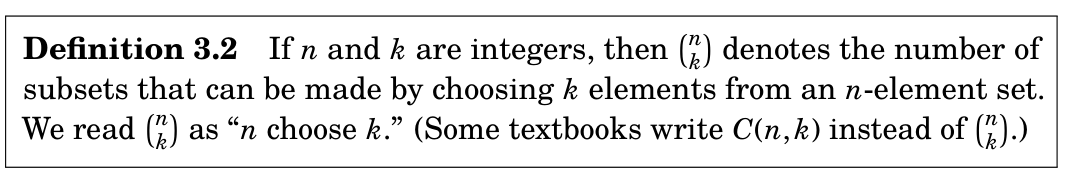
\includegraphics[width=0.9\textwidth]{images/definition03_02.png}
\end{figure}

\begin{figure}
	\centering
	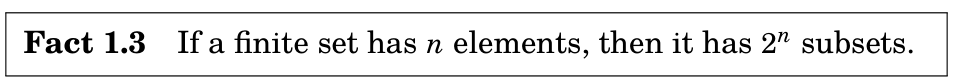
\includegraphics[width=0.9\textwidth]{images/fact01_03.png}
\end{figure}

\begin{exercise}{}{}
	Use the binomial theorem to show the following.
	\begin{alist}
		\item
		$$\sum\limits_{k=0}^n 3^k \binom{n}{k}=4^n$$
		\item
		The binomial theorem asserts the following.
		$$
			(x+y)^n = \sum\limits_{k=0}^n \dbinom{n}{k} x^{n-k}y^k
		$$
		\item Let $x=1, y=3$, then
		$$
			(1+3)^n = \sum\limits_{k=0}^n \dbinom{n}{k} 1^{n-k}3^k
		$$
		$$
			4^n = \sum\limits_{k=0}^n \dbinom{n}{k} 3^k
		$$
	\end{alist}
\end{exercise}


\begin{exercise}{}{}
	Use Fact 3.5 (page 87) to derive Equation 3.3 (page 90).
	\begin{alist}
		\item First let's expand out the right hand side, and get a common denominator.
		$$\dbinom{n}{k-1} =\dfrac{n!}{(k-1)!(n-k+1)!}$$
		$$=\dfrac{n!}{(k-1)!(n-k)!(n-k+1)} =\dfrac{kn!}{k(k-1)!(n-k)!(n-k+1)}$$

		$$\dbinom{n}{k}=\dfrac{n!}{k!(n-k)!}=
			\dfrac{n!}{k(k-1)!(n-k)!}=
			\dfrac{(n-k+1)n!}{(n-k+1)k(k-1)!(n-k)!}
		$$

		$$\dbinom{n}{k-1} + \dbinom{n}{k}=$$
		$$ \dfrac{kn!+(n-k+1)n!}{(n-k+1)k(k-1)!(n-k)!}=
			\dfrac{n!(k+n-k+1)}{(n-k+1)!k!}= $$
		$$ \dfrac{n!(n+1)}{(n-k+1)!k!}=
			\dfrac{(n+1)!}{(n-k+1)!k!}= \dbinom{n+1}{k}$$
	\end{alist}
\end{exercise}

\begin{figure}
	\centering
	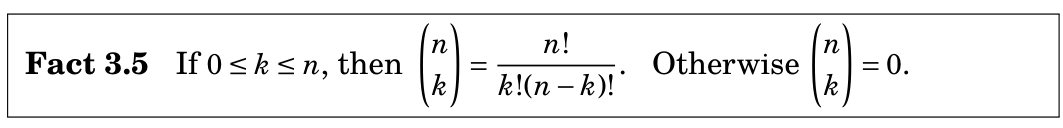
\includegraphics[width=0.9\textwidth]{images/fact03_05.png}
\end{figure}
\begin{figure}
	\centering
	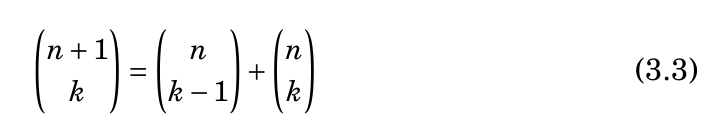
\includegraphics[width=0.9\textwidth]{images/equation03_03.png}
\end{figure}

\begin{exercise}{}{}
	Use the binomial theorem to show
	\begin{alist}
		\item
		$$
			\dbinom{n}{0}
			- \dbinom{n}{1}
			+ \dbinom{n}{2}
			- \dbinom{n}{3}
			+ \dbinom{n}{4}
			\dots
			+ (-1)^n\dbinom{n}{n} =0, \quad n>0.
		$$
		\item The binomial theorem states
		$$(x+y)^n=\sum\limits_{i=0}^n\dbinom{n}{i}x^{n-i}y^i$$
		$$
			\dbinom{n}{0}
			- \dbinom{n}{1}
			+ \dbinom{n}{2}
			- \dbinom{n}{3}
			+ \dbinom{n}{4}
			\dots
			+ (-1)^n\dbinom{n}{n}=(1+(-1))^n = 0^n = 0
		$$
	\end{alist}
\end{exercise}

\begin{exercise}{}{}
	Show that the formula $k\dbinom{n}{k}=n\dbinom{n-1}
		k-1$
	is true for all integers $n, k$ with $0 \leq k \leq n$.
	\begin{alist}
		\item Suppose $k\neq0$
		$$k\dbinom{n}{k}=n\dbinom{n-1}{k-1}$$
		$$k\dfrac{n!}{(n-k)!k!}=n\dfrac{(n-1)!}{(k-1)!(n-1-k+1)!}$$
		$$k\dfrac{n!}{(n-k)!k!}=\dfrac{n!}{(k-1)!(n-k)!}$$
		$$k\dfrac{n!}{(n-k)!k!}=\dfrac{n!}{(k-1)!(n-k)!}\cdot\dfrac{k}{k}$$
		$$k\dfrac{n!}{(n-k)!k!}=k\dfrac{n!}{(n-k)!k!}$$
		\item Suppose $k=0$
		$$0\cdot\dbinom{n}{0}=n\dbinom{n-1}{-1}$$
		$$0\cdot\dbinom{n}{0}=n\cdot 0$$
		$$0=0$$
	\end{alist}
\end{exercise}

\begin{exercise}{}{}
	Use the binomial theorem to show
	\begin{alist}
		\item
		$$9^n=\sum\limits_{k=0}^{n} (-1)^k\dbinom{n}{k}10^{n-k}$$
		\item The binomial theorem states
		$$(x+y)^n=\sum\limits_{i=0}^n\dbinom{n}{i}x^{n-i}y^i$$
		\item let $x=-1, y=10$
		$$((-1)+10)^n=\sum\limits_{k=0}^{n} (-1)^k\dbinom{n}{k}10^{n-k}$$
	\end{alist}
\end{exercise}

\begin{exercise}{}{}
	Show that
	$$
		\dbinom{n}{k}
		\dbinom{k}{m}=
		\dbinom{n}{m}
		\dbinom{n-m}{k-m}
	$$
	\begin{alist}
		\item
		$$
			\dbinom{n}{k}
			\dbinom{k}{m}=
			\dfrac{n!}{(n-k)!k!}
			\dfrac{k!}{(m-k)!m!}=
			\dfrac{n!}{(n-k)!(m-k)!m!}
		$$
		$$
			\dbinom{n}{m}
			\dbinom{n-m}{k-m}=
			\dfrac{n!}{(n-m)!m!}\cdot
			\dfrac{(n-m)!}{(k-m)!(n-m-k+m)!}=
		$$
		$$
			\dfrac{n!}{m!}\cdot
			\dfrac{1}{(k-m)!(n-k)!}=\dfrac{n!}{(n-k)!(m-k)!m!}
		$$
	\end{alist}
\end{exercise}

\begin{exercise}{}{}
	Show that
	\begin{alist}
		\item
		$$
			\dbinom{n}{3}=
			\dbinom{2}{2} +
			\dbinom{3}{2} +
			\dbinom{4}{2} +
			\dbinom{5}{2} +
			\dots +
			\dbinom{n-1}{2}
		$$

		\item Remember this equality:
		$$\dbinom{n+1}{k} = \dbinom{n}{k} + \dbinom{n}{k-1}$$

		\item The binomial theorem states
		$$(x+y)^n=\sum\limits_{i=0}^n\dbinom{n}{i}x^{n-i}y^i$$
		\item

		\item Suppose $k=3$
		$$
			\dbinom{n}{3}=
			\dbinom{n-1}{2} +
			\dbinom{n-1}{3}
		$$
		$$
			\dbinom{n-1}{3} =
			\dbinom{n-2}{2} +
			\dbinom{n-2}{3}
		$$
		$$
			\dbinom{n-2}{3} =
			\dbinom{n-3}{2} +
			\dbinom{n-3}{3}
		$$
		$$
			\dots
		$$
	\end{alist}
\end{exercise}
\begin{figure}
	\centering
	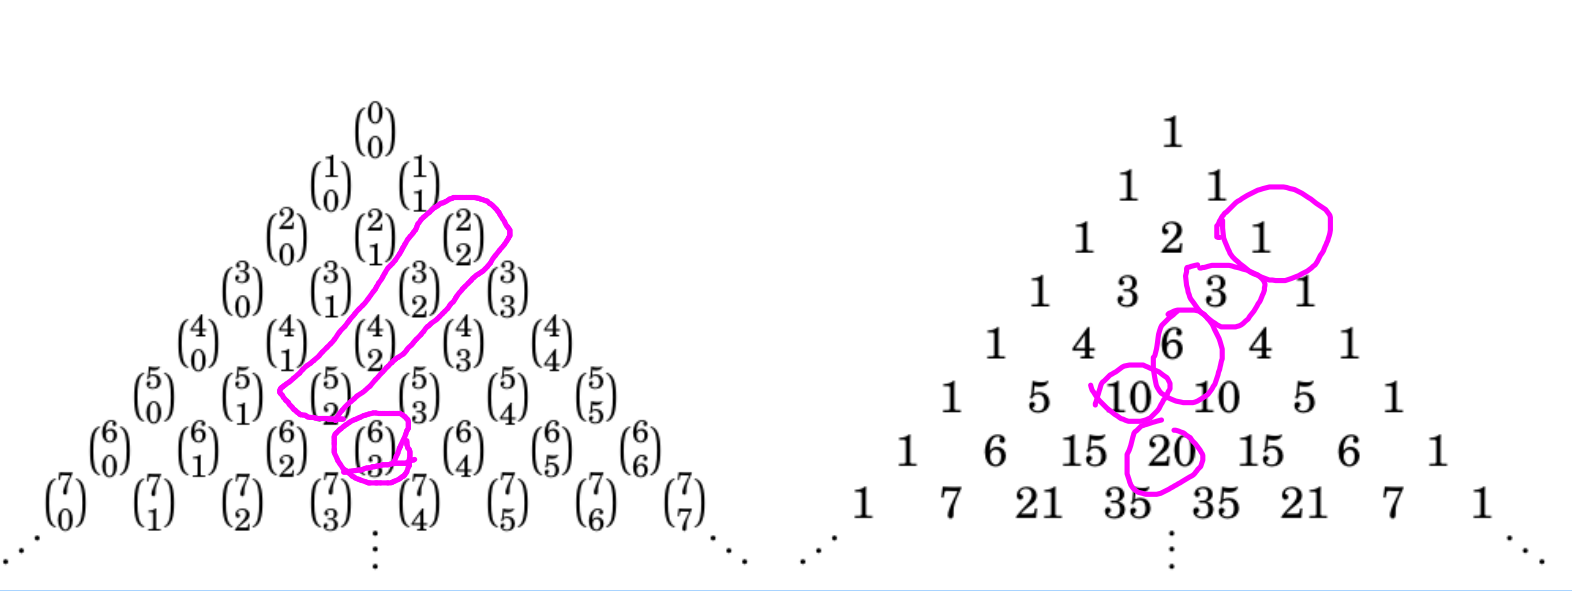
\includegraphics[width=0.7\textwidth]{images/pascals-triangle.png}
\end{figure}
\begin{exercise}{}{}
	The first five rows of Pascal's triangle appear in the digits of powers of 11: 110 = 1,
	111 = 11, 112 = 121, 113 = 1331 and 114 = 14641. Why is this so? Why does the
	pattern not continue with 115?
\end{exercise}

\section{Inclusion Exclusion}

\begin{exercise}{}
	At a certain university 523 of the seniors are history
	majors or math majors (or both). There are 100 senior math majors, and 33
	seniors are majoring in both history and math. How many seniors are majoring in
	history?
	\begin{alist}
		\item Let $A=$ math majors, $|A|=100$
		\item Let $B=$ history majors
		\item $A\cap B=$ both history and math major, $|A\cap B|=33$
		\item $A \cup B$ =math or history majors or both, $|A\cup B|=|A| +
			|B| - |A\cap B|=523$
		\item
		$$|A\cup B|=|A| + |B| - |A\cap B|=523$$
		$$|B| = 523 + |A\cap B| - |A|$$
		$$|B| = 523 + 33 - 100$$
		$$|B| = 456$$
	\end{alist}
\end{exercise}

\begin{exercise}{}{}
	How many 4-digit positive integers are there for which
	there are no repeated digits, or for which there may be repeated digits, but
	all digits are odd?
	\begin{alist}
		\item Let $A=$ 4-digit positive integers
		\item Let $B=$ 4-digit positive integers with no repeated digits, $B \subset
			A$
		\item Let $C=$ 4-digit positive integers with repeated digits and all digits
		are odd, $C \subset A$
		\item $C\cap B$  = 4-digit positive integers for which there are
		no repeated digits and all digits are odd.
		\item $C\cup B$  = 4-digit positive integers for which there are
		no repeated digits, or for which there may be repeated digits, but all
		digits are odd.
		\item
		$$|C\cup B| = |C| + |B| - |C\cap B|$$
		\item For B, we can pick any number 1..9 to start, and then for each
		subsequent digit we can pick between 0..9, excluding the one that came
		before, therefore there are also 9 choices for each non-starting digit.
		$|B| = 9^4$.
		\item For C, we can pick any number 1,3,5,7,9 for all 4 positions, therefore
		$|C|=5^4$.
		\item For $|C\cap B|$, we can pick any number 1,3,5,7,9 for the first
		position, and thereafter we can pick from any of the odd digits that did
		not directly precede the current one, therefore there are $|C \cap
			B|=5\cdot4^3$.
		\item $$|C\cup B| = |C| + |B| - |C\cap B|$$
		\item $$|C\cup B| = 5^4+9^4-5\cdot 4^3$$
	\end{alist}
\end{exercise}

\begin{exercise}{}{}
	How many 4-digit positive integers are there that are even or contain no 0's?
	\begin{alist}
		\item Let $A=$ 4-digit positive integers that are even
		\item Let $B=$ 4-digit positive integers that contain no zeros
		\item $A \cap B=$ 4-digit positive integers that are even and contain no zeros
		\item $A \cup B=$ 4-digit positive integers that are even or contain no zeros
		\item To create elements in A, we can pick 1..9 to start, then 0..9 for the
		second and third digits, and any of the 5 even digits for the last
		digit, therefore $|A|=9\cdot 10^2\cdot5$.
		\item To create elements in B, we can pick from 1..9 for all digits,
		therefore $|B|=9^4$.
		\item To create elements in $A\cap B$, we can pick from 1..9 for the first
		3 digits and 2,4,6,8 for the last digit, therefore $|A\cap B|=9^3\cdot4$
		\item $$|A\cup B| = |A| + |B| - |A\cap B|$$
		\item $$|A\cup B| = 9\cdot10^2\cdot5 + 9^4 - 9^3\cdot4$$
	\end{alist}
\end{exercise}

\begin{exercise}{}{}
	This problem involves lists made from the letters T, H, E, O, R, Y, with repetition allowed.
	\begin{alist}
		\item (a) How many 4-letter lists are there that don't begin with T, or don't
		end in Y?
		\item Let $A=$ 4-letter lists that dont begin with T
		\item Let $B=$ 4-letter lists that dont end with Y
		\item Let $A\cap B=$ 4-letter lists that dont begin with T and dont end with Y
		\item Let $A\cup B=$ 4-letter lists that dont begin with T or dont end with Y
		\item $|A|= 5\cdot6\cdot6\cdot6$
		\item $|B|= 6\cdot6\cdot6\cdot5$
		\item $|A\cap B|= 5\cdot6\cdot6\cdot5$
		\item $|A\cup B|= |A| + |B| - |A\cap B| = 2\cdot 6^3\cdot5 - 5^2\cdot6^2$
		\item (b) How many 4-letter lists are there in which the sequence of letters T,
		H, E appears consecutively (in that order)?
		\item Other than THE, there is one letter-spot left free, and there are 6 letters
		available for that spot. THE can be placed starting at either position 1 or
		position 2 for a total of two choices. Therefore by the multiplication
		principle there are $2\cdot6$ 4-letter lists matching the problem criteria.
		\item (c) How many 6-letter lists are there in which the sequence of letters T,
		H, E appears consecutively (in that order)?
		\item Other than THE, there are three letter-spots left free, and there are 6 letters
		available for those 3 spots. THE can be placed starting at either position
		1, 2, 3, or 4 for a total of four choices. Therefore by the multiplication
		principle there are $4\cdot6^3$ 6-letter lists matching the problem criteria.
	\end{alist}
\end{exercise}

\begin{exercise}{}{}
	How many 7-digit binary strings begin in 1 or end in 1 or have exactly four 1's?
	\begin{alist}
		\item Let $A=$ 7-digit binary strings that begin in 1
		\item Let $B=$ 7-digit binary strings that end in 1
		\item Let $C=$ 7-digit binary strings that have exactly four 1s
		\item Let $D=$ 7-digit binary strings
		\item $A\cup B \cup C=$ 7-digit binary strings begin in 1 or end in 1 or have exactly four 1's
		\item $\neg(A\cup B \cup C)=\neg A \cap \neg B \cap \neg C=$
		7-digit binary strings dont begin in 1 and dont end in 1 and dont have
		exactly four 1's.
		\item To create elements of $\neg A \cap \neg B \cap \neg C$,
		the first and last digit must be 0. For the middle 5 spots, there must
		be either 0, 1, 2, 3, or 5 1s. This means there are
		$\binom{5}{0}+\binom{5}{1}+\binom{5}{2}+\binom{5}{3}+\binom{5}{5}$ ways
		to arrange the middle 5 spots.
		\item We can use the fact that $A\cup B \cup C$ is the complement of
		$\neg(A\cup B \cup C)$ to determine that
		$$|D| - |\neg(A\cup B \cup C)|=| A\cup B \cup C |$$
		$$ | A\cup B \cup C | = 2^7 - \binom{5}{0}-\binom{5}{1}-\binom{5}{2}-\binom{5}{3}-\binom{5}{5}$$
	\end{alist}
\end{exercise}

\begin{exercise}{}{}
	Is the following statement true or false? Explain. If
	$A_1
		\cap A_2 \cap A_3 =\emptyset$ , then $|A_1 \cup A_2 \cup A_3| =
		|A_1|+|A_2|+|A_3|$.

	\begin{alist}
		\item
		$$
			A_1 \cap A_2 \cap A_3 =\emptyset
			\implies
			|A_1 \cup A_2 \cup A_3| = |A_1|+|A_2|+|A_3|
		$$
		\item Suppose $A_1 \cap A_2 \cap A_3 =\emptyset$.
		\item Let
		$A_1=\{1, 2\},\quad
			A_2=\{1, 3\},\quad
			A_3=\{4, 5\} $
		\item This is a counter-example as $|A_1 \cup A_2 \cup A_3|=5$ while
		$|A_1|+|A_2|+|A_3| = 2 +2 +2=6$.
		\item For the implication to hold, we must also know that intersection between
		any two of the sets is also the empty-set.
	\end{alist}
\end{exercise}

\begin{exercise}{}{}7. Consider 4-card hands dealt off of a standard 52-card deck.
	How many hands are there for which all 4 cards are of the same suit or all 4
	cards are red?
	\begin{alist}
		\item Let $A=$ all 4 cards are the same suit
		\item Let $B=$ all 4 cards are red
		\item $A\cap B=$ all 4 cards are same suit AND all 4 cards are red
		\item $A\cup B=$ all 4 cards are same suit OR all 4 cards are red
		\item
		$$
			|A \cup B | = |A| + |B| - |A \cap B|
		$$
		\item $|A| = 4\cdot\dbinom{13}{4}$
		\item $|B| = \dbinom{26}{4}$
		\item $|A\cap B| = 2\cdot\dbinom{13}{4}$
		\item
		$$
			|A \cup B | = 4\cdot\dbinom{13}{4} + \dbinom{26}{4} - 2\cdot\dbinom{13}{4}
		$$
	\end{alist}
\end{exercise}

\begin{exercise}{}{}
	Consider 4-card hands dealt off of a standard 52-card deck.
	How many hands are there for which all 4 cards are of different suits or all
	4 cards are red?
	\begin{alist}
		\item Let $A=$ all 4 cards are of different suit
		\item Let $B=$ all 4 cards are red
		\item $A\cap B=\emptyset$ all 4 cards are different suit and all 4 cards are red
		\item $|A| = \dfrac{13^4}{4!}$
		\item $|B| = \dbinom{26}{4}$
		\item
		$$
			|A \cup B | = |A| + |B| - |A \cap B|
			|A \cup B | = \dfrac{13^4}{4!} + \dbinom{26}{4} - 0
		$$
	\end{alist}
\end{exercise}

\begin{exercise}{}{}
	A 4-letter list is made from the letters L, I, S, T, E, D
	according to the following rule: Repetition is allowed, and the first two
	letters on the list are vowels or the list ends in D. How many such lists are
	possible?
	\begin{alist}
		\item Let $A=$ first two letters on the list are vowels
		\item Let $B=$ the list ends in D
		\item $A\cap B=$ first two letters on the list are vowels and the list ends in D
		\item $A\cup B=$ first two letters on the list are vowels or the list ends in D
		\item To determine $|A|$, we note that there are $2^2$ to pick the first two
		letters as vowels, and then $6^4$ possibilities for the next four letters.
		\item To determine $|B|$, the last letter is fixed, and there $6^5$
		possibilities for the first 5 letters.
		\item To determine $|A\cap B|$ there are $2^2$ possibilities for the first two
		letters as vowel, the last letter is fixed, and the middle 3 letters have
		$6^3$ possible arrangements.
		\item Therefore
		$$|A \cup B | = |A| + |B| - |A \cap B|$$
		$$|A \cup B | = 2^2\cdot6^4 + 6^5 - 2^2\cdot6^3$$
	\end{alist}
\end{exercise}

\begin{exercise}{}{}
	How many 6-digit numbers are even or are divisible by 5?
	\begin{alist}
		\item let $a=$ 6-digit numbers that are even
		\item let $b=$ 6-digit numbers that are divisible by 5
		\item $a\cap b=$ 6-digit numbers that are even and divisible by 5
		\item $a\cup b=$ 6-digit numbers that are even or divisible by 5
		\item $|a|=9\cdot10^4\cdot5$
		\item $|b|=9\cdot10^4\cdot2$
		\item $|a\cap b|= 9\cdot10^4\cdot1$
		\item $$|a\cup b|= 9\cdot10^4\cdot5 + 9\cdot10^4\cdot2 - 9\cdot10^4\cdot1$$
		\item $$= (9\cdot10^4)(5 + 2 -1)$$
		\item $$= 54\cdot10^4$$
	\end{alist}
\end{exercise}

\begin{exercise}{}{}
	How many 7-digit numbers are even or have exactly three digits equal to 0?
	\begin{alist}
		\item let $a=$ 7-digit numbers that are even
		\item let $b=$ 7-digit numbers that have exactly three digits equal to 0
		\item $a\cap b=$ 7-digit numbers that are even and have exactly three digits equal to 0
		\item $a\cup b=$ 7-digit numbers that are even or have exactly three digits equal to 0
		\item $|a|=9\cdot10^6\cdot5$
		\item to calculate $|b|$, we note that there must be three 0s, and because we
		can't start the number with 0, there are $\dbinom{6}{3}$ possible choices of
		where to place them. for the remaining 4 digits, there are
		9 choices for the first digit and $10^3$ for the remaining choices. then by the multiplication principle, there are
		$|b|=9\cdot10^3\cdot \dbinom{6}{3}$.
		\item to calculate $|a\cap b|$, we consider two different cases. in the first
		case, the number ends with 0, therefore there are two zeros to place in 5
		spots. the first digit has 9 choices, the non-zeroes have $10^3$ choices,
		and so $9\cdot\dbinom{5}{2}\cdot10^3$. possibilties for this case. for the
		second case that does not end with a zero, there are 9 choices for the
		first digit, $\dbinom{5}{3}$ for the zeros, and 4 choices for the last
		digit, and $10^2$ for the remaining digits. therefore there are
		$9\cdot\dbinom{5}{3}\cdot10^2\cdot4$ for the second case. the cases sum together for
		$9\cdot\dbinom{5}{3}\cdot10^2\cdot4 +
			9\cdot\dbinom{5}{2}\cdot10^3$ total choices from $|a\cap b|$.
		\item therefore
		$$|a \cup b | = |a| + |b| - |a \cap b|$$
		$$|a \cup b | =
			9\cdot10^6\cdot5 + 9\cdot10^3\cdot \dbinom{6}{3} - 9\cdot\dbinom{5}{3}\cdot10^2\cdot4 - 9\cdot\dbinom{5}{2}\cdot10^3$$
	\end{alist}
\end{exercise}

\begin{exercise}{}{}
	12. How many 5-digit numbers are there in which three of the
	digits are 7, or two of the digits are 2?
	\begin{alist}
		\item Let $A=$ 5-digit numbers in which at least three of the digits are 7
		\item Let $B=$ 5-digit numbers in which at least two of the digits are 2
		\item $A\cap B= $ 5-digit numbers in which two of the digits are 2 AND three are 7
		\item $A\cup B= $ 5-digit numbers in which two of the digits are 2 OR three are 7

		\begin{itemize}
			\item 5 7s = If there are 5 7's, there is only way to create that digit. $1$
			\item 4 7s = If there are 4 7's, there are 8 ways to create that digit if
			      the number does not start with 7, and $\dbinom{4}{3}\cdot9$ ways if it
			      does start with 7.
			\item 3 7s = If there are 4 7's, there are 8 ways to create that digit if
			      the number does not start with 7, and $\dbinom{4}{3}\cdot9$ ways if it
			      does start with 7.
		\end{itemize}

		\item $|A|$, case 1, where it begins with 7. Then the remaining 7s can go in
		$\dbinom{4}{2}$ spots, and the remaining two digits have $9^2$ choices.
		\item $|A|$, case 1, where it does not begin with 7. There are 8 choices for the
		first digit (exclude 0 and 7), $\dbinom{4}{3}$ spots for the 7s, and 9 spots
		for the remaining digit.

		\item didnt finish. These problems are becoming a grind ...
	\end{alist}
\end{exercise}

% % 13. How many 8-digit binary strings end in 1 or have exactly four 1's?
% % 14. How many 3-card hands (from a standard 52-card deck) have the property that
% % it is not the case that all cards are black or all cards are of the same suit?
% % 15. How many 10-digit binary strings begin in 1 or end in 1?

\section{Counting Multisets}
\begin{exercise}{}{}
	How many 10-element multisets can be made from the symbols $\set{1,2,3,4}$?
	\begin{alist}
		\item Let $X= \{ 1,2,3,4\}$, and $|X|=4$.
		\item Let $Y=$ a multiset of cardinality 10.
		\item The total permutations of a k-multiset constructed from a set with
		n-cardinality is
		$$ \dbinom{k+n-1}{k} = \dbinom{k+n-1}{n-1} $$
		\item For this problem $k=10, n=4$.
		\item Therefore there are $\binom{13}{4}$ possible 10-element multisets made
		from the symbols $1\dots4$.
	\end{alist}
\end{exercise}

\begin{exercise}{}{}
	2. How many 2-element multisets can be made from the 26 letters of the alphabet?
	\begin{alist}
		\item Let $A=$ 26 letter alphabet.
		\item Let $Y=$ a multiset of cardinality 2.
		\item For this problem, $k=2, n=26$
		$$ \dbinom{k+n-1}{k} = \dbinom{k+n-1}{n-1} $$
		$$ \dbinom{27}{2}$$
		$$ \dfrac{27!}{25!\cdot2!}$$
		$$ \dfrac{26\cdot27}{2}$$
	\end{alist}
\end{exercise}

\begin{exercise}{}{}
	You have a dollar in pennies, a dollar in nickels, a dollar in dimes, and a dollar in quarters. You give a friend four coins. How many ways can this be done?
	\begin{alist}
		\item Let the set $A= \{a_1, a_2, a_3, a_4\}$, where $a_i$ is a coin type.
		\item The question is equivalent to: given a set of cardinality 4, how many
		different multisets of cardinality 4 can be created?
		\item The information about the different number of starting coins is
		irrelevant other than assuring there are at least $k=4$ of each coin.
		\item Therefore the answer is the following
		$$ \dbinom{k+n-1}{k} $$
		$$ \dbinom{7}{4}$$
	\end{alist}
\end{exercise}

\begin{exercise}{}{}
	A bag contains 20 identical red balls, 20 identical blue
	balls, 20 identical green balls, and 20 identical white balls. You reach in
	and grab 15 balls. How many different outcomes are possible?
	\begin{alist}
		\item This question is asking about how many multisets can be created from
		an initial set. Let $a_i$ be the number of starting balls for color $i$.
		Let $k$ be the cardinality of the desired multiset. As long as $a_i\geq k$,
		then all possible multisets can be created.
		\item Therefore the answer is the following
		$$ \dbinom{k+n-1}{k} $$
		$$ \dbinom{15+4-1}{15}$$
		$$ \dbinom{18}{15}$$
	\end{alist}
\end{exercise}

\begin{exercise}{}{}
	A bag contains 20 identical red balls, 20 identical blue balls, 20 identical
	green balls, and one white ball. You reach in and grab 15 balls. How many
	different outcomes are possible?
	\begin{alist}
		\item Let $A$=multiset of 15 of colored balls, from 3 colors
		\item Let $B$=multiset of 14 of colored balls, from 3 colors
		\item Let $C$=multisets of 15 of colored balls starting from 20
		identical red balls, 20 identical blue balls, 20 identical green balls, and
		one white ball.
		\item We can partition $C$ into two sets: those with a white ball and those
		without a white ball. For the first partition, it is the same as asking how
		many multisets of cardinality 14 can be created from a set of 3 balls, which
		is represented by $B$. The second partition is the same as asking how many
		multisets of size 15 can be created from a set of 3 balls, which is
		represented by $A$.
		\item Therefore $C=A \cup B$, and $|C| = |A| + |B|$.
		\item
		$$ |A| = \dbinom{k+n-1}{k} = \dbinom{15+3-1}{15}=\dbinom{17}{15}$$
		$$ |B| = \dbinom{k+n-1}{k} = \dbinom{14+3-1}{14}=\dbinom{16}{14}$$
		$$ |C| = 256 $$
	\end{alist}
\end{exercise}

\begin{exercise}{}{}A bag contains 20 identical red balls, 20 identical blue
	balls, 20 identical green balls, one white ball, and one black ball. You
	reach in and grab 20 balls. How many different outcomes are possible?
	\begin{alist}
		\item Case 1, 0 white balls, 0 black balls, $k=20, n=3$
		$$ \dbinom{k+n-1}{k} = \dbinom{20+3-1}{20}=\dbinom{22}{20}$$
		\item Case 2, 0 white balls, 1 black ball , $k=19, n=3$
		$$ \dbinom{k+n-1}{k} = \dbinom{19+3-1}{19}=\dbinom{21}{19}$$
		\item Case 3, 1 white ball, 0 black balls, $k=19, n=3$
		$$ \dbinom{k+n-1}{k} = \dbinom{19+3-1}{19}=\dbinom{21}{19}$$
		\item Case 4, 1 white ball, 1 black ball, $k=18, n=3$
		$$ \dbinom{k+n-1}{k} = \dbinom{18+3-1}{18}=\dbinom{20}{18}$$
		\item Therefore the answer is
		$$ \dbinom{22}{20} +\dbinom{21}{19} +\dbinom{21}{19} +\dbinom{20}{18}$$
	\end{alist}
\end{exercise}

\begin{exercise}{}{}
	In how many ways can you place 20 identical balls into five
	different boxes?
	\begin{alist}
		\item This is a stars-and-bars type problem, which is the equivalent of asking,
		given a finite set X with cardinality $n$, how many multisets of cardinality
		$k$ can be created? Here the cardinality of X is 5, and k=20.
		\item Therefore the answer is
		$$ \dbinom{k+n-1}{k} = \dbinom{20+5-1}{20}=\dbinom{24}{20}$$
	\end{alist}
\end{exercise}

\begin{exercise}{}{}
	How many lists (x, y, z) of three integers are there with
	$0 \leq x \leq y \leq z \leq 100$?
	\begin{alist}
		\item  Imagine 100 stars, and then placing 2 bars somewhere within them. This
		transforms the problems into asking how many multisets of cardinality 100
		can be created from a set of cardinality 3, which is solved by the
		following.
		$$ \dbinom{100+3-1}{100} = \dbinom{102}{100}$$
	\end{alist}
\end{exercise}

\begin{exercise}{}{}
	A bag contains 50 pennies, 50 nickels, 50 dimes and 50 quarters. You reach
	in and grab 30 coins. How many different outcomes are possible?
	\begin{alist}
		\item Let $p_i$ be the count of count $i$. There are sufficient coins such that
		$\forall i, p_i\geq k$, where $k$ is the cardinality of the desired
		multiset.
		\item There there are this many possible outcomes, where $n$ is the cardinality
		of the distinct coin set.
		$$ \dbinom{k+n-1}{k} = \dbinom{4+30-1}{30}=\dbinom{33}{30}$$
	\end{alist}
\end{exercise}

\begin{exercise}{}{}
	How many non-negative integer solutions does $$u + v+ w+ x+
		y+ z = 90$$ have?
	\begin{alist}
		\item Suppose a set of 90 stars.  We can partition those stars 6 times with 5
		bars, and then we will have transformed the original problem into an
		equivalent formulation stated as: how many multisets of cardinality 90 can
		be created from an initial set of cardinality 6, which is calculated as
		follows.
		$$ \dbinom{90+6-1}{90} = \dbinom{95}{90}$$
	\end{alist}
\end{exercise}

\begin{exercise}{}{}
	How many integer solutions does the equation
	$w + x + y+ z = 100$ have if $w \geq 4, x \geq 2, y \geq 0, z \geq 0$?
	\begin{alist}
		\item Let A = solutions to the problem
		$$w + x + y+ z = 100, w \geq 0, x \geq 0, y \geq 0, z \geq 0$$.
		\item Let $B=w<4$ and $C=x<2$. From the set $|A|$, we must delete all solutions
		where $B\lor C$. So we are left with determining the cardinality of the
		solution set $B \lor C$, which is equal to
		$$
			|B\lor C| = |B| + |C| - |B\land C|
		$$
		\item To determine $|B|$ solve this problem
		$$w + x + y+ z = 100, \neg(w \geq 4), x \geq 0, y \geq 0, z \geq 0$$
		$$\implies x + y+ z = 97, x \geq 0, y \geq 0, z \geq 0$$

		\item To determine $|C|$ solve this problem
		$$w + x + y+ z = 100, w \geq 0, \neg(x \geq 2), y \geq 0, z \geq 0$$
		$$\implies w + y+ z = 99, w \geq 0, y \geq 0, z \geq 0$$

		\item To determine $|B\land C|$ solve this problem
		(w, x)
		(0, 0)
		(0, 1)
		(1, 0)
		(1, 1)
		(2, 0)
		(2, 1)
		(3, 0)
		(3, 1)
		\item There's a much simpler approach.
	\end{alist}
\end{exercise}

\begin{exercise}{}{}
	How many integer solutions does the equation
	$$w + x + y+ z = 100, w \geq 7, x \geq 0, y \geq 5, z \geq 4$$
	\begin{alist}
		\item This problem is the same as
		$$w + x + y+ z = 84, w \geq 0, x \geq 0, y \geq 0, z \geq 0$$
		\item Therefore the solution is calculated with $k=84, n=4$ as
		$$ \dbinom{k+n-1}{k} = \dbinom{84+4-1}{84}=\dbinom{87}{84}$$
	\end{alist}
\end{exercise}

\begin{exercise}{}{}
	How many length-6 lists can be made from the symbols $\{a,
		b, c, d, e, f, g\}$, if repetition is allowed and the list is in
	alphabetical order? (Examples: bbcegg, but not bbbagg.)
	\begin{alist}
		\item Creating lists is equivalent to counting permutations. Only allowing lists
		in some order is equivalent to counting multisets. Therefore this problem
		can be restated in an equivalent form as---how many cardinality 6 multisets
		can be created from an original set of cardinality 7.
		\item This can be calculated as the following, with $k=6, n=7$.
		$$ \dbinom{k+n-1}{k} = \dbinom{6+7-1}{6}=\dbinom{12}{6}$$
	\end{alist}
\end{exercise}

\begin{exercise}{}{}
	How many permutations are there of the letters in the word “PEPPERMINT”?
	\begin{alist}
		\item This problem is the equivalent to asking---given a multiset, how many
		permutations can be made.  We must know the cardinality of the multiset, and each
		the multiplicity of each element from the underlying set.
		\item Then the permutation can be calculated as follows
		$$ \dfrac{n!}{\Pi{p_i}!} = \dfrac{10!}{3!2!}$$
	\end{alist}
\end{exercise}

\begin{exercise}{}{}
	How many permutations are there of the letters in the word “TENNESSEE”?
	\begin{alist}
		\item The permutation can be calculated as follows $$
			\dfrac{n!}{\Pi{p_i}!} = \dfrac{9!}{4!2!2!}$$
	\end{alist}
\end{exercise}

\begin{exercise}{}{}
	A community in Canada's Northwest Territories is known in the local language
	as “TUKTUYAAQTUUQ.” How many permutations does this name have?
	\begin{alist}
		\item
		4 U
		3 T
		2 Q
		2 A
		1 Y
		1 K
		\item The permutations can be calculated as follows $$
			\dfrac{n!}{\Pi{p_i}!} = \dfrac{13!}{4!3!2!2!}$$
	\end{alist}
\end{exercise}

\begin{exercise}{}{}
	You roll a dice six times in a row. How many possible outcomes are there
	that have two 1's three 5's and one 6?
	\begin{alist}
		\item We begin with the multiset $\{1, 1, 5, 5, 5, 6\}$. We must determine how
		many permutations there are of this multiset.
		\item The permutation can be calculated as follows
		$$ \dfrac{n!}{\Pi{p_i}!} = \dfrac{6!}{2!3!}$$
	\end{alist}
\end{exercise}

\begin{exercise}{}{}
	Flip a coin ten times in a row. How many outcomes have 3 heads and 7 tails?
	\begin{alist}
		\item We begin with the multiset of 3 heads and 7 tails. We must determine how
		many permutations there are of this multiset.
		\item The permutation can be calculated as follows
		$$ \dfrac{n!}{\Pi{p_i}!} = \dfrac{10!}{7!3!}$$
	\end{alist}
\end{exercise}

\begin{exercise}{}{}
	In how many ways can you place 15 identical balls into 20
	different boxes if each box can hold at most one ball?
	\begin{alist}
		\item This can be encoded as a selection problem. We are choose 15 of the boxes
		to hold a single ball.
		\item Therefore this can be calculated with
		$$ \dbinom{20}{15}$$
	\end{alist}
\end{exercise}

\begin{exercise}{}{}
	You distribute 25 identical pieces of candy among five children. In how many
	ways can this be done?
	\begin{alist}
		\item This can be encoded as stars and bars problem. Given a finite set of 5
		children, how many multisets of cardinality 25 can be made?
		\item This can calculated with $n=5, k=25$
		$$ \dbinom{k+n-1}{k} = \dbinom{25+5-1}{29}=\dbinom{29}{25}$$
	\end{alist}
\end{exercise}

\begin{exercise}{}{}
	How many numbers between 10,000 and 99,999 contain one or more of the digits
	3, 4 and 8, but no others?
	\begin{alist}
		\item Starting with the finite set $\{3, 4, 8\}$, how many multisets of
		cardinality 5 can be constructed? This is not a multiset problem, as that
		would imply an ordering on the digits, whereas for example 34444 and 43444
		should be counted separately, which would not happen with a multiset.
		\item This can calculated with $n=3, k=5$
		$$ \dbinom{k+n-1}{k} = \dbinom{3+5-1}{5}=\dbinom{7}{5}$$
	\end{alist}
\end{exercise}

\section{Division and Pigeonhole Principles}

\begin{exercise}{}{}
	Show that if six integers are chosen at random, then at
	least two of them will have the same remainder when divided by 5.
	\begin{alist}
		\item Let $A=\{0, 1, 2, 3, 4\}$, and for any $i\in\mathbb{Z}, i\mod 5 \in
			A$.
		\item The division principle states that for $n, k\in \mathbb{N}$, if $n$
		objects are placed in $k$ slots, then at least one box contains
		$\up{\dfrac{n}{k}}$ or more objects. Here $|A|=k=5$, and $n=6$.
		\item Therefore at least $\up{\dfrac{n}{k}}=\up{\dfrac{6}{5}}=2$
		two of the randomly chosen integers mod 5 are the same value.
	\end{alist}
\end{exercise}

\begin{exercise}{}{}
	You deal a pile of cards, face down, from a standard
	52-card deck. What is the least number of cards the pile must have before
	you can be assured that it contains at least five cards of the same suit?
	\begin{alist}
		\item The division principle states that for $n, k\in \mathbb{N}$, if $n$
		objects are placed in $k$ slots, then at least one box contains
		$\up{\dfrac{n}{k}}$ or more objects
		\item Each suit is a slot. We need to calculate the number of cards needed
		$n$ such that $\up{\dfrac{n}{k}}>=5$.
		\item Because $k=4$, then $n=17$.
	\end{alist}
\end{exercise}

\begin{exercise}{}{}
	What is the fewest number of times you must roll a
	six-sided dice before you can be assured that 10 or more of the rolls
	resulted in the same number?
	\begin{alist}
		\item The division principle states that for $n, k\in \mathbb{N}$, if $n$
		objects are placed in $k$ slots, then at least one box contains
		$\up{\dfrac{n}{k}}$ or more objects
		\item Each dice-face is a slot. We need to calculate the number of rolls needed
		$n$ such that $\up{\dfrac{n}{k}}>=10$.
		\item Because $k=6$, then $n=k\cdot(10 -1)+ 1 = 55$.
	\end{alist}
\end{exercise}

\begin{exercise}{}{}
	Select any five points on a square whose side-length is one
	unit. Show that at least two of these points are within $\frac{\sqrt{2}}{2}$
	units of each other.

	\begin{alist}
		\item Divide the square into four equal subsquares with side length
		$\frac{1}{2}$, and notice that the diagonal of each subsquare has a length
		of $\frac{\sqrt{2}}{2}$.
		\item Since we have 5 points and only 4 subsquares, at least two points must lie
		in the same subsquare by the pigeonhole principle.
		\item By the nature of the subsquare, the maximum distance between any two
		points within the same subsquare is the diagonal length, which is
		$\frac{\sqrt{2}}{2}$.
		\item Therefore, at least two of the five points are within $\frac{\sqrt{2}}{2}$
		units of each other.
	\end{alist}
\end{exercise}

\begin{exercise}{}{}
	Prove that any set of seven distinct natural numbers
	contains a pair of numbers whose sum or difference is divisible by 10.

	\begin{alist}
		\item Consider the final digit $d$ of some $a \in \mathbb{N}$.
		\item $d$ will be in 0..9.
	\end{alist}
\end{exercise}

\begin{exercise}{}{}
	Given a sphere S, a great circle of S is the intersection
	of S with a plane through its center. Every great circle divides S into two
	parts. A hemisphere is the union of the great circle and one of these two parts.
	Show that if five points are placed arbitrarily on S, then there is a hemisphere
	that contains four of them.
	\begin{alist}
		\item Use two points to define a great circle, which also creates two
		hemispheres.
		\item Three points remain, which by the pigeonhole principle means, one
		hemisphere has two points of those points, and the other has one.
		\item The points used to construct the great circle can be considered part of
		the hemisphere with 2 points, therefore that hemisphere has 4 points.
	\end{alist}
\end{exercise}

\section{Combinatorial Proofs}
\begin{exercise}{}{}
	Show that
	$$1(n-0)+2(n-1)+3(n-2)+4(n-3)+\dots+(n-1)2+(n-0)1 = \binom{n+2}{3}$$ .
	\begin{alist}
		\item The expression $\binom{n+2}{3}$ is equivalent to the ways we can select
		size-3 subsets from a set of size $(n+2)$.
		$$
			n+2n-2+3n-6+4n-12+\dots+2n-2+n = \binom{n+2}{3}
		$$

		$$
			\binom{n+2}{3}=
			\dfrac{(n+2)!}{3!(n-1)!}=
			\dfrac{(n+2)(n+1)(n)(n-1)!}{3!(n-1)!}=
			\dfrac{(n+2)(n+1)(n)}{6}=
		$$

		$$
			\binom{n+2}{3} = \binom{n+1}{3} + \binom{n+1}{2}
		$$
	\end{alist}
	yeah, no idea. see solution
\end{exercise}

\begin{exercise}{}{}
	Show that $1 + 2 + 3 + \dots + n = \binom{n+1}{2}$.
	\begin{alist}
		\item Let $A=\{0, 1, ... n\}$, which has cardinality $n+1$.  From this set we'll
		choose subsets of size 2.
		$$
			\binom{n+1}{2} =
			\dfrac{(n+1)!}{2!(n-1)!} =
			\dfrac{(n+1)n(n-1)!}{2!(n-1)!} =
			\dfrac{n^2+n}{2}
		$$
		\item We can pair together $n+0$, $(n-1) + 1$, $(n-2) + 2$, etc such that we
		have $\dfrac{n}{2}\cdot n$, and one middle element which is $\dfrac{n}{2}$.
		\item Therefore we have shown that $1 + 2 + 3 + \dots + n = \binom{n+1}{2}$.
	\end{alist}
\end{exercise}

\begin{exercise}{}{}
	Show that
	$$ \dbinom{n}{2} \dbinom{n-2}{k-2}= \dbinom{n}{k} \dbinom{k}{2} $$
	\begin{alist}
		\item
		$$ \dfrac{n!}{2!(n-2)!} \dfrac{(n-2)!}{(k-2)!(n-2-k+2)!}=
			\dfrac{n!}{k!(n-k)!} \dfrac{k!}{2!(k-2)!} $$
		\item
		$$ \dfrac{n!}{2!} \dfrac{1}{(k-2)!(n-2-k+2)!}= \dfrac{n!}{(n-k)!} \dfrac{1}{2!(k-2)!} $$
		\item
		$$ \dfrac{n!}{2(k-2)!(n-k)!}= \dfrac{n!}{(n-k)!2(k-2)!} $$
	\end{alist}
\end{exercise}

\begin{exercise}{}{}
	Show that $P(n,k) = P(n-1,k)+ k \cdot P(n-1,k -1)$.
	\begin{alist}
		\item
		$$ P(n,k) = \dfrac{n!}{(n-k)!}$$
		$$ P(n-1,k) =  \dfrac{(n-1)!}{(n-1-k)!}\cdot\dfrac{n-k}{n-k} =\dfrac{(n-k)(n-1)!}{(n-k)!}
		$$
		$$ k\cdot P(n-1,k -1) = \dfrac{k(n-1)!}{(n-k)!}$$
		$$ P(n-1,k)+ k \cdot P(n-1,k -1) = \dfrac{(n-k+k)(n-1)!}{(n-k)!} =
			\dfrac{n!}{(n-k)!}
		$$
		\item There is surely some fancy, less grunt-mole way of solving this.
	\end{alist}
\end{exercise}

breaking my brain, pausing this here.

\part{How to Prove Conditional Statements}
\part{More on Proof}
\part{Relations, Functions, and Cardinality}
% \printbibliography{}
% \printindex{}
\end{document}
